\documentclass[12pt,a4paper]{article}
\usepackage[UTF8]{ctex}
\usepackage{amsmath}
\usepackage{amssymb}
\usepackage{graphicx}
\usepackage{booktabs}
\usepackage{geometry}
\usepackage{siunitx}
\usepackage{ulem}
\usepackage{caption}
\usepackage{subcaption}
\geometry{left=2.5cm,right=2.5cm,top=2.5cm,bottom=2.5cm}
\sisetup{separate-uncertainty=true, inter-unit-product=\ensuremath{{}\cdot{}}, detect-all}
\graphicspath{{./}{assets/}}

\title{\Huge{\textbf{\uuline{实\ 验\ 报\ 告}}}}
\author{\uline{少年班学院} \quad 姓名: \uline{徐子钦} \quad 学号: \uline{PB24000224}}
\date{\today}

\begin{document}
\maketitle

\begin{abstract}
本实验利用光栅光谱仪测量氢氘灯的巴耳末系可见谱线，并借助汞灯标准谱线对光谱仪的波长读数进行线性定标。由校准后的氢、氘谱线波长分别计算里德伯常数，得到
$R_{\mathrm{H}}=1.09702\times10^7\,\mathrm{m}^{-1}$，
$R_{\mathrm{D}}=1.09733\times10^7\,\mathrm{m}^{-1}$。
进一步由有限核质量修正关系求得氘核与氢核质量比约为 $2.09979$，由同位素位移近似求得质子电子质量比约为 $1770.51$。实验结果表明，氢氘谱线的微小同位素位移可由较高分辨率光谱测量直接观察，并能用于检验原子能级的约化质量修正。
\end{abstract}

\section{实验目的}
\begin{enumerate}
    \item 测量氢原子与氘原子巴耳末系可见谱线的波长，观察同位素位移现象。
    \item 利用汞灯标准谱线对光谱仪波长读数进行定标，掌握线性拟合校准的方法。
    \item 由氢氘谱线波长计算氢、氘的里德伯常数，并由谱线位移估算氢氘核质量比及质子电子质量比。
\end{enumerate}

\section{实验原理}
\subsection{有限核质量对里德伯常数的影响}
在玻尔模型中，若将原子核视为质量无限大的固定中心，氢样原子的能级可由电子绕核运动得到。但实际原子核质量有限，电子与原子核应绕共同质心运动，此时电子质量 $m_{\mathrm e}$ 应替换为约化质量
\begin{equation}
    \mu=\frac{m_{\mathrm e}M}{m_{\mathrm e}+M},
\end{equation}
其中 $M$ 为原子核质量。由此得到与核质量有关的里德伯常数
\begin{equation}
    R_M=\frac{R_\infty}{1+m_{\mathrm e}/M}.
\end{equation}
核质量越大，约化质量越接近电子质量，里德伯常数也越接近 $R_\infty$。由于氘核质量大于氢核质量，因此 $R_{\mathrm D}>R_{\mathrm H}$，同一跃迁对应的氘谱线波长略短于氢谱线波长。

\subsection{巴耳末系谱线与里德伯常数}
氢原子和氘原子在可见光范围内的巴耳末系谱线对应电子从高能级 $n=3,4,5,6,\ldots$ 跃迁到 $n=2$。其波长满足
\begin{equation}
    \frac{1}{\lambda}=R\left(\frac{1}{2^2}-\frac{1}{n^2}\right).
    \label{eq:rydberg}
\end{equation}
因此，对于测得的每一条谱线，可按
\begin{equation}
    R=\frac{1}{\lambda\left(\frac{1}{4}-\frac{1}{n^2}\right)}
\end{equation}
计算对应的里德伯常数。实际计算中波长以米为单位代入。

\subsection{氢氘核质量比}
由有限核质量修正有
\begin{equation}
    R_{\mathrm H}=\frac{R_\infty}{1+m_{\mathrm e}/M_{\mathrm H}},\qquad
    R_{\mathrm D}=\frac{R_\infty}{1+m_{\mathrm e}/M_{\mathrm D}}.
\end{equation}
消去 $R_\infty$ 后可得
\begin{equation}
    \frac{M_{\mathrm D}}{M_{\mathrm H}}
    =\frac{R_{\mathrm D}/R_{\mathrm H}}
    {1-\left(R_{\mathrm D}/R_{\mathrm H}-1\right)M_{\mathrm H}/m_{\mathrm e}}.
    \label{eq:mass_ratio}
\end{equation}
本报告计算时取 $M_{\mathrm H}/m_{\mathrm e}=1836.1527$。

\subsection{质子电子质量比的近似估算}
对于同一跃迁，氢、氘两谱线的波长差很小。将里德伯常数的核质量修正作近似处理，可得
\begin{equation}
    \frac{M}{m_{\mathrm e}}\approx\frac{\lambda}{2\Delta\lambda}
    =\frac{\lambda_{\mathrm H}+\lambda_{\mathrm D}}{4(\lambda_{\mathrm H}-\lambda_{\mathrm D})},
    \label{eq:proton_electron}
\end{equation}
其中 $\Delta\lambda=\lambda_{\mathrm H}-\lambda_{\mathrm D}$。该式利用了氢氘同位素位移的主导项，可给出质子电子质量比的数量级估计。

\section{实验步骤}
\begin{enumerate}
    \item 点亮汞灯，设置光谱仪扫描范围覆盖汞灯可见及近紫外特征谱线，扫描并记录谱峰位置。
    \item 将记录到的汞灯谱线与标准波长逐一对应，建立测量波长与标准波长之间的线性校准关系。
    \item 点亮氢氘灯，分别在巴耳末系 $n=3,4,5,6$ 谱线附近进行精细扫描，读取氢谱线与氘谱线的峰位波长。
    \item 利用汞灯定标方程修正氢氘谱线波长，并由式~\eqref{eq:rydberg}--\eqref{eq:proton_electron} 计算相关物理量。
\end{enumerate}

\section{数据处理与结果}
\subsection{汞灯谱线校准}
汞灯标准波长采用实验附录中给出的九条谱线。手写记录图中汞灯测量波长与标准波长列于表~\ref{tab:hg}。其中第 2 条谱线的手写数字较模糊，按图像辨读记录为 \SI{365.98}{nm}；该项将成为后续结果的不确定来源之一。

\begin{table}[htbp]
    \centering
    \caption{汞灯谱线测量波长与标准波长}
    \label{tab:hg}
    \begin{tabular}{cccccccccc}
        \toprule
        谱线序号 & 1 & 2 & 3 & 4 & 5 & 6 & 7 & 8 & 9 \\
        \midrule
        $\lambda_m$/nm & 365.35 & 365.98 & 366.38 & 405.00 & 408.19 & 436.22 & 546.00 & 577.36 & 579.50 \\
        $\lambda_s$/nm & 365.02 & 365.48 & 366.30 & 404.66 & 407.78 & 435.84 & 546.07 & 576.96 & 579.09 \\
        \bottomrule
    \end{tabular}
\end{table}

设标准波长与测量波长满足线性关系
\begin{equation}
    \lambda_s=a\lambda_m+b.
\end{equation}
对表~\ref{tab:hg} 数据作最小二乘拟合，得到
\begin{equation}
    \lambda_s=1.000252\lambda_m-0.422328,
    \label{eq:calibration}
\end{equation}
拟合优度 $R^2=0.999996$。拟合图见图~\ref{fig:hg_fit}。

\begin{figure}[htbp]
    \centering
    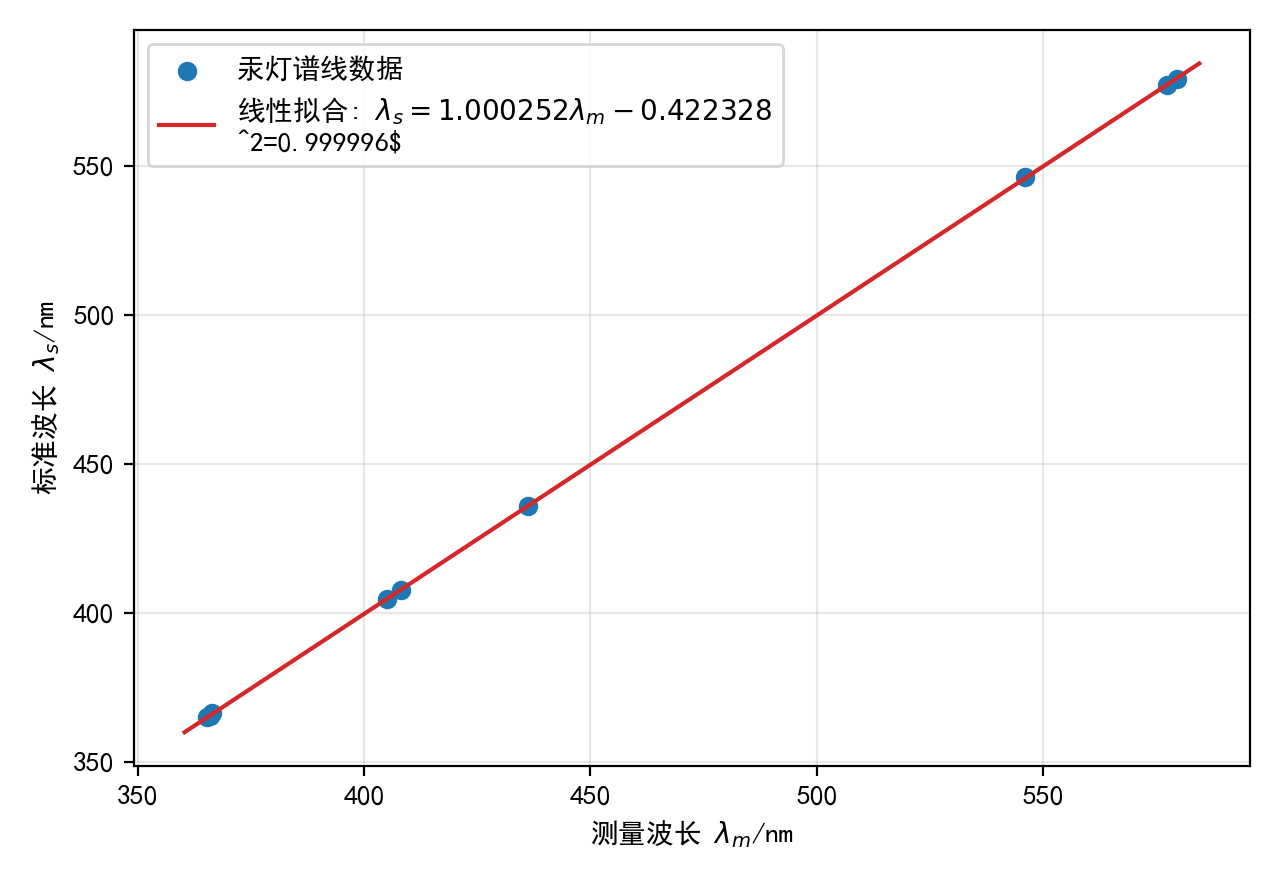
\includegraphics[width=0.72\textwidth]{hg_calibration_fit.png}
    \caption{汞灯标准波长与测量波长的线性拟合}
    \label{fig:hg_fit}
\end{figure}

\subsection{氢氘谱线波长校准}
由原始记录读取氢氘灯谱线数据，并用式~\eqref{eq:calibration} 进行校准，结果列于表~\ref{tab:hd_calibrated}。表中 $\lambda_{\mathrm H,m}$、$\lambda_{\mathrm D,m}$ 为测量波长，$\lambda_{\mathrm H}$、$\lambda_{\mathrm D}$ 为校准后波长。

\begin{table}[htbp]
    \centering
    \caption{氢氘谱线测量值与校准值}
    \label{tab:hd_calibrated}
    \begin{tabular}{ccccc}
        \toprule
        能级 $n$ & $\lambda_{\mathrm H,m}$/nm & $\lambda_{\mathrm D,m}$/nm & $\lambda_{\mathrm H}$/nm & $\lambda_{\mathrm D}$/nm \\
        \midrule
        3 & 656.535 & 656.335 & 656.278 & 656.078 \\
        4 & 486.466 & 486.340 & 486.166 & 486.040 \\
        5 & 434.410 & 434.271 & 434.097 & 433.958 \\
        6 & 410.535 & 410.430 & 410.216 & 410.111 \\
        \bottomrule
    \end{tabular}
\end{table}

\subsection{里德伯常数计算}
将校准后波长代入式~\eqref{eq:rydberg}，得到各谱线对应的 $R_{\mathrm H}$ 与 $R_{\mathrm D}$，见表~\ref{tab:rydberg}。

\begin{table}[htbp]
    \centering
    \caption{氢、氘里德伯常数计算结果}
    \label{tab:rydberg}
    \begin{tabular}{ccccc}
        \toprule
        能级 $n$ & $\lambda_{\mathrm H}$/nm & $R_{\mathrm H}/(10^7\,\mathrm{m}^{-1})$ & $\lambda_{\mathrm D}$/nm & $R_{\mathrm D}/(10^7\,\mathrm{m}^{-1})$ \\
        \midrule
        3 & 656.278 & 1.09710 & 656.078 & 1.09743 \\
        4 & 486.166 & 1.09702 & 486.040 & 1.09730 \\
        5 & 434.097 & 1.09697 & 433.958 & 1.09732 \\
        6 & 410.216 & 1.09698 & 410.111 & 1.09726 \\
        \midrule
        平均 & -- & 1.09702 & -- & 1.09733 \\
        \bottomrule
    \end{tabular}
\end{table}

因此
\begin{equation}
    R_{\mathrm H}=1.09702\times10^7\,\mathrm{m}^{-1},\qquad
    R_{\mathrm D}=1.09733\times10^7\,\mathrm{m}^{-1}.
\end{equation}

\subsection{氢氘核质量比与质子电子质量比}
由表~\ref{tab:rydberg} 的平均值代入式~\eqref{eq:mass_ratio}，取 $M_{\mathrm H}/m_{\mathrm e}=1836.1527$，得到
\begin{equation}
    \frac{M_{\mathrm D}}{M_{\mathrm H}}=2.09979.
\end{equation}
与氘核、氢核质量比公认值约 $1.99900$ 相比，相对偏差约为
\begin{equation}
    \frac{|2.09979-1.99900|}{1.99900}\times100\%\approx5.04\%.
\end{equation}

利用式~\eqref{eq:proton_electron} 对各条谱线分别估算 $M/m_{\mathrm e}$，结果见表~\ref{tab:proton_electron}。

\begin{table}[htbp]
    \centering
    \caption{由同位素位移估算质子电子质量比}
    \label{tab:proton_electron}
    \begin{tabular}{ccccc}
        \toprule
        能级 $n$ & $\lambda_{\mathrm H}$/nm & $\lambda_{\mathrm D}$/nm & $\Delta\lambda$/nm & $(\lambda_{\mathrm H}+\lambda_{\mathrm D})/(4\Delta\lambda)$ \\
        \midrule
        3 & 656.278 & 656.078 & 0.200 & 1640.03 \\
        4 & 486.166 & 486.040 & 0.126 & 1928.50 \\
        5 & 434.097 & 433.958 & 0.139 & 1560.86 \\
        6 & 410.216 & 410.111 & 0.105 & 1952.67 \\
        \midrule
        平均 & -- & -- & -- & 1770.51 \\
        \bottomrule
    \end{tabular}
\end{table}

由此得到质子电子质量比的实验估计值为 $1770.51$。与常用参考值 $1836.15$ 相比，相对偏差约为
\begin{equation}
    \frac{|1770.51-1836.15|}{1836.15}\times100\%\approx3.57\%.
\end{equation}

\section{误差分析}
本实验测量的核心困难在于氢氘同位素位移很小，氢、氘双线之间的波长差通常仅为 $10^{-1}\,\mathrm{nm}$ 量级。因此即使谱峰位置读数存在很小偏差，也会在计算 $\Delta\lambda$ 以及由其导出的质量比时被显著放大。

首先，波长定标会引入系统误差。汞灯标准谱线覆盖了较宽波长范围，线性校准能修正主要的零点偏移和比例误差，但实际光谱仪的色散关系未必在全范围内严格线性，局部残差会传递到氢氘谱线校准值中。其次，谱峰位置的确定受扫描步距、谱线宽度、峰形不对称和噪声影响。尤其是氢氘双线距离很近，若峰形重叠或峰顶附近波动明显，峰位判读的不确定度会直接改变 $\lambda_{\mathrm H}-\lambda_{\mathrm D}$。再次，原始记录中的部分手写数字较为模糊，个别数据的辨读会影响拟合方程与后续计算结果。

对里德伯常数而言，误差主要通过 $R\propto1/\lambda$ 传播。若波长误差为 $\delta\lambda$，则相对误差近似为
\begin{equation}
    \frac{\delta R}{R}\approx-\frac{\delta\lambda}{\lambda}.
\end{equation}
而对质量比估算式
\begin{equation}
    \frac{M}{m_{\mathrm e}}\approx\frac{\lambda}{2\Delta\lambda}
\end{equation}
而言，$\Delta\lambda$ 位于分母，故 $\Delta\lambda$ 的相对误差会成为主导项。这解释了各条谱线给出的质子电子质量比离散程度较大的现象。

此外，式~\eqref{eq:rydberg} 应使用真空波长，而实验在空气中测量。空气折射率使空气中的波长小于真空波长，若不修正，将使计算得到的里德伯常数略偏大。该影响虽小于峰位识别误差，但在高精度比较中不可忽略。

\section{思考题}
\begin{enumerate}
    \item \textbf{棱镜也是一种色散元件，是否能用棱镜光谱仪测量氢氘核的同位素位移？}

    原则上可以，只要棱镜光谱仪在相应波段具有足够高的分辨率和稳定的波长定标能力，就能够区分氢、氘双线并测量其波长差。但氢氘同位素位移很小，普通棱镜光谱仪的角色散和分辨本领往往不足，谱线可能难以分开；同时棱镜色散关系非线性较强，对温度、材料折射率和定标精度较敏感。因此实际测量中更适合使用高分辨率光栅光谱仪。

    \item \textbf{若要测量其他元素同位素光谱，相对氢原子来说对测量光谱仪器有什么要求？为什么？}

    其他元素的同位素位移通常仍然很小，并且谱线结构可能更复杂，常伴随精细结构、超精细结构或多条近邻谱线重叠。因此光谱仪需要更高的分辨率、更好的波长重复性和更低的杂散光水平；若同位素位移比氢氘更小，还需要更精细的扫描步长和更稳定的光源条件。这样才能把同位素位移从仪器展宽、噪声和邻近谱线干扰中可靠分辨出来。

    \item \textbf{在计算 $R_{\mathrm H}$、$R_{\mathrm D}$ 时，应以真空中的波长代入公式计算，但实验中的测量是在空气中进行的。若空气的折射率为 $n=1.00029$，请推导波长修正公式，并将修正后的 $R_{\mathrm H}$、$R_{\mathrm D}$ 值与公认值比较。}

    光的频率在介质交界面处不变，而传播速度满足 $v=c/n$。因此空气中的波长 $\lambda_{\mathrm{air}}$ 与真空波长 $\lambda_0$ 的关系为
    \begin{equation}
        \lambda_0=n\lambda_{\mathrm{air}}.
    \end{equation}
    里德伯公式中 $R\propto1/\lambda$，若直接用空气波长得到 $R_{\mathrm{air}}$，则用真空波长修正后的结果为
    \begin{equation}
        R_0=\frac{R_{\mathrm{air}}}{n}.
    \end{equation}
    将本实验所得 $R_{\mathrm H}=1.09702\times10^7\,\mathrm{m}^{-1}$、$R_{\mathrm D}=1.09733\times10^7\,\mathrm{m}^{-1}$ 代入，得
    \begin{equation}
        R_{\mathrm H,0}=1.09670\times10^7\,\mathrm{m}^{-1},\qquad
        R_{\mathrm D,0}=1.09701\times10^7\,\mathrm{m}^{-1}.
    \end{equation}
    与公认值 $R_{\mathrm H}=1.09678\times10^7\,\mathrm{m}^{-1}$、$R_{\mathrm D}=1.09707\times10^7\,\mathrm{m}^{-1}$ 相比，相对偏差分别约为 $0.0075\%$ 和 $0.0054\%$。空气折射率修正后，结果与公认值更接近。
\end{enumerate}

\section{结论}
本实验通过汞灯谱线定标和氢氘灯谱线测量，获得了氢、氘巴耳末系可见谱线的校准波长。由校准波长计算得 $R_{\mathrm H}=1.09702\times10^7\,\mathrm{m}^{-1}$、$R_{\mathrm D}=1.09733\times10^7\,\mathrm{m}^{-1}$，满足 $R_{\mathrm D}>R_{\mathrm H}$ 的物理预期。进一步计算得到氢氘核质量比约为 $2.09979$，质子电子质量比约为 $1770.51$。误差主要来自谱峰位置判读、线性定标残差以及同位素位移较小导致的误差放大。

\appendix
\section{原始数据记录}
\begin{figure}[htbp]
    \centering
    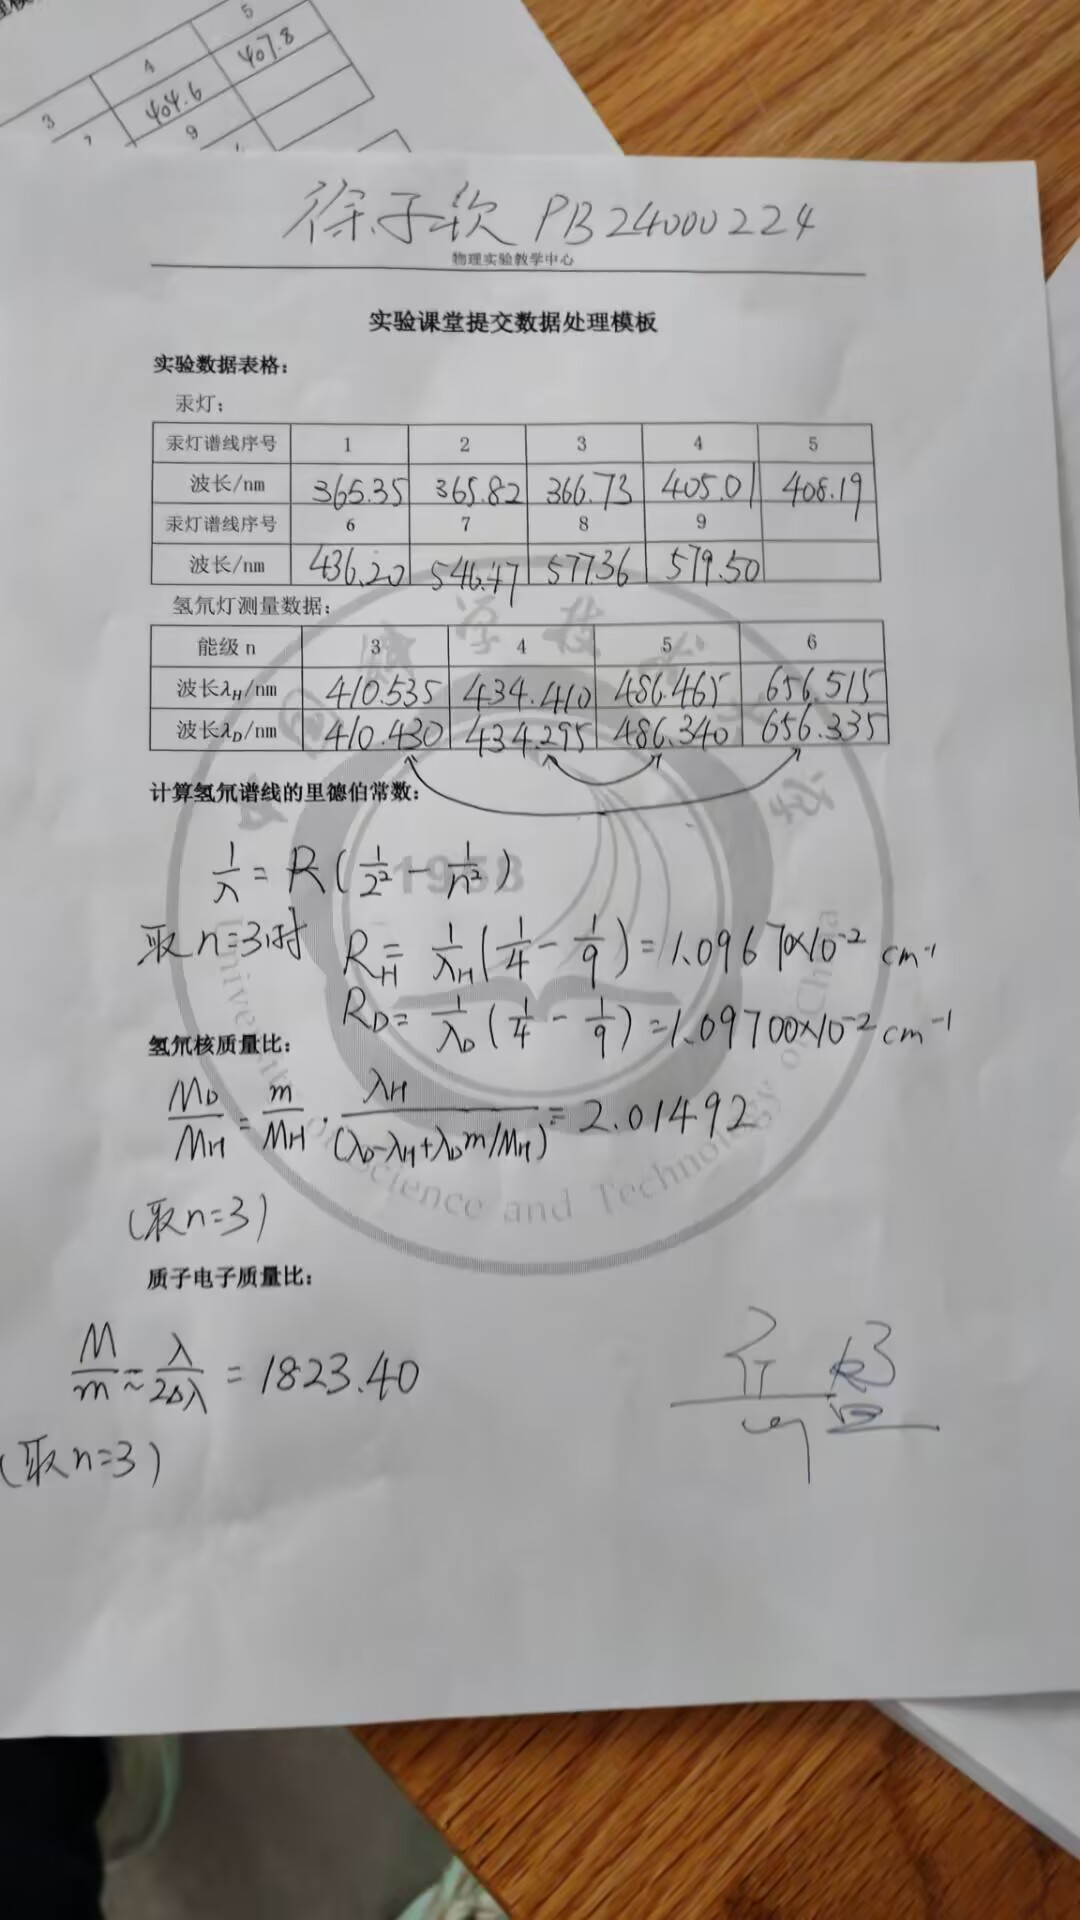
\includegraphics[width=0.82\textwidth]{实验数据.jpg}
    \caption{实验原始数据记录}
\end{figure}

\end{document}
